% Drawing 69/01-6 -- folder 69, batch 01, archive page 6 (PDF page 7).
% Transcription: à gauche, deux figures en perspective : un prisme de sommets $x$, $y$, $s$, $t$ en bas et $\xi$, $\xi'$, $\eta$, $\eta'$ en haut ; au-dessous, une seconde figure, plus grande, sur les mêmes lettres, en partie couverte de hachures
% Kind: prism in perspective and a larger overwritten figure. Method 2 (schematic redraw from the facsimile). Status: partial.
% Notes: Upper figure: eight vertices placed once, every edge drawn between them: the face xi, xi', t, x on top (xi at the top left, xi' at the top right, x at the left, t inside), the edges xi -- s and t -- y inked heavier (drawn thick), x -- s, s -- y, xi' -- y, x -- eta, eta -- eta', s -- eta', y -- eta', and a short hidden stroke down from t. Letters placed where they stand on the page (xi, xi', x, t, y, s, eta, eta'); which letter belongs to which vertex is the page's, not checked against the text. Lower figure: the larger version, eight vertices with the thick strokes (the vertical edge through the top, the two edges to the right vertex, the long thick diagonal from the left vertex), two short hidden strokes. Still differs from the facsimile: the lower figure is covered with scribbles (the transcription's hachures, which strike it); they are not drawn. Its letters are placed where they stand on the page: eta, eta' above, t at the right, x inside, s at the left, y at the lower right, xi, xi' under the two lower vertices; they are partly overwritten. Redrawn 2026-11-09 (issue 128): vertices placed once and every edge drawn between them, labels at \small, strike-outs not drawn; to check again.
% Coordinates: 1 unit = 1 mm = 1/100 of the crop width (bbox in page fractions: [0.1, 0.56, 0.32, 0.8]).
% Redrawn by Claude (claude-opus-5-5), issue #73, 2026-11-09; not checked by a human; not compiled (no TeX in the session).
% Rights: reproduces part of the work -- behind RENDER_TRANSCRIPTS, never published by itself.
\documentclass[tikz,border=3pt]{standalone}
\usepackage{amsmath,amssymb}
\usetikzlibrary{patterns,arrows.meta}
\tikzset{pencil/.style={black!45}, struck/.style={black!35}, mark/.style={circle,draw,inner sep=1.3pt}, pt/.style={circle,fill,inner sep=0.9pt}, opt/.style={circle,draw,fill=white,inner sep=1.1pt}}
\begin{document}
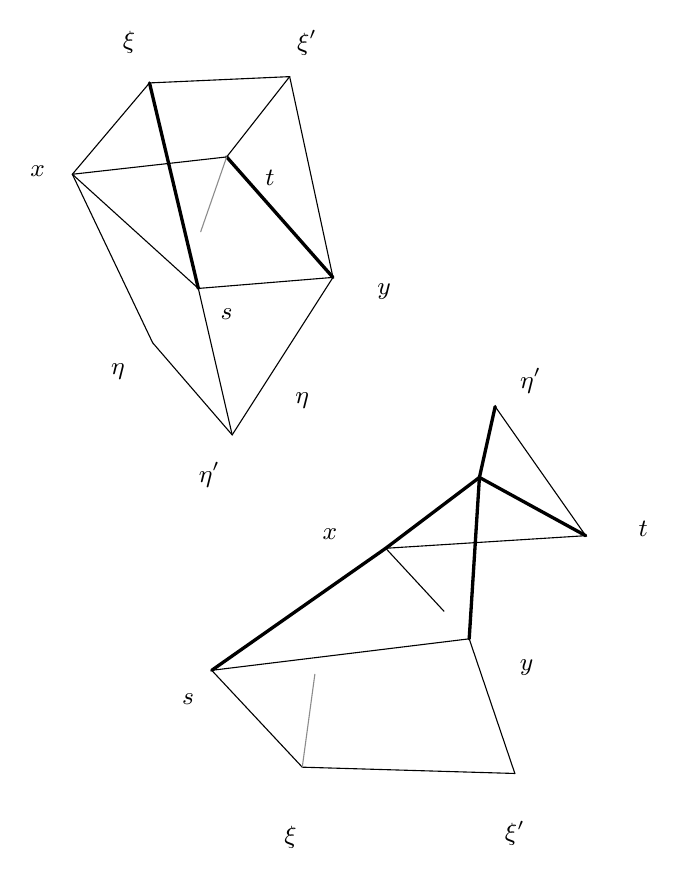
\begin{tikzpicture}[x=1mm,y=1mm,line cap=round,line join=round,font=\scriptsize]
\draw (31.1,-19.2) -- (48.9,-18.4);
\draw (31.1,-19.2) -- (21.3,-30.8);
\draw (21.3,-30.8) -- (40.9,-28.6);
\draw (40.9,-28.6) -- (48.9,-18.4);
\draw (48.9,-18.4) -- (54.4,-43.9);
\draw[very thick] (40.9,-28.6) -- (54.4,-43.9);
\draw[very thick] (31.1,-19.2) -- (37.3,-45.3);
\draw (21.3,-30.8) -- (37.3,-45.3);
\draw (37.3,-45.3) -- (54.4,-43.9);
\draw (21.3,-30.8) -- (31.5,-52.2);
\draw (31.5,-52.2) -- (41.6,-63.9);
\draw (37.3,-45.3) -- (41.6,-63.9);
\draw (54.4,-43.9) -- (41.6,-63.9);
\draw[pencil] (40.9,-28.6) -- (37.6,-38.1);
\node[inner sep=1pt] at (28.5,-14.1) {\small $\xi$};
\node[inner sep=1pt] at (51.1,-14.1) {\small $\xi'$};
\node[inner sep=1pt] at (16.9,-30.4) {\small $x$};
\node[inner sep=1pt] at (46.4,-31.2) {\small $t$};
\node[inner sep=1pt] at (60.9,-45.7) {\small $y$};
\node[inner sep=1pt] at (40.9,-48.6) {\small $s$};
\node[inner sep=1pt] at (27.1,-55.9) {\small $\eta$};
\node[inner sep=1pt] at (38.7,-69) {\small $\eta'$};
\draw[very thick] (75,-60.3) -- (73,-69.3) -- (71.7,-89.8);
\draw (75,-60.3) -- (86.5,-76.7);
\draw[very thick] (73,-69.3) -- (86.5,-76.7);
\draw (61.1,-78.3) -- (86.5,-76.7);
\draw[very thick] (61.1,-78.3) -- (73,-69.3);
\draw[very thick] (39,-93.8) -- (61.1,-78.3);
\draw (39,-93.8) -- (71.7,-89.8);
\draw (39,-93.8) -- (50.5,-106.1);
\draw (50.5,-106.1) -- (77.5,-106.9);
\draw (71.7,-89.8) -- (77.5,-106.9);
\draw (61.1,-78.3) -- (68.5,-86.3);
\draw[pencil] (50.5,-106.1) -- (52.1,-94.3);
\node[inner sep=1pt] at (93.8,-75.8) {\small $t$};
\node[inner sep=1pt] at (36,-97.5) {\small $s$};
\node[inner sep=1pt] at (79,-93.5) {\small $y$};
\node[inner sep=1pt] at (49,-115) {\small $\xi$};
\node[inner sep=1pt] at (77.5,-114.5) {\small $\xi'$};
\node[inner sep=1pt] at (50.5,-59.5) {\small $\eta$};
\node[inner sep=1pt] at (79.5,-57) {\small $\eta'$};
\node[inner sep=1pt] at (54,-76.5) {\small $x$};
\end{tikzpicture}
\end{document}
